%%%%%%%%%%%%%%%%%%%%%%%%%%%%%%%%%%%%%%%%%%%%%%%%%%%%%%%%%%%%%%%%%%%%%%
%%                       IAEW LaTeX Template                        %%
%%%%%%%%%%%%%%%%%%%%%%%%%%%%%%%%%%%%%%%%%%%%%%%%%%%%%%%%%%%%%%%%%%%%%%

\chapter{Exemplarische Anwendung und Ergebnisse}
\label{ch:results}
% ===============================================================
% NEUE SORTIERUNG vom 18.09.2026. Grundlage ist KAPITEL_4_AUFBAU.md im
% Wurzelverzeichnis, Abschnitte 4 und 5. Die alte Gliederung vom 18.08.2026
% steht vollstaendig am Ende dieser Datei als Kommentar. Sie ist nicht wieder
% aufzunehmen, weil ihre Abschnitte 4.1 und 4.2 inzwischen in Abschnitt 3.3
% und in den Anhaengen zur Einzelmarktvalidierung und zum Fahrplan ohne die
% Mindestgroesse stehen.
%
% STICHPUNKTPHASE nach WORKFLOW.md Abschnitt 3. Die itemize-Bloecke sind
% Stichpunkte, ein Stichpunkt je spaeterem Satz. Fliesstext entsteht erst nach
% einem vom Verfasser freigegebenen Absatzplan. Die Zeile NICHT SAGEN ist nach
% WORKFLOW.md Abschnitt 7 fuer jeden Absatzplan dieses Kapitels Pflicht.
%
% Zielumfang Kapitel 4: 16 Seiten
%   Kapiteleinleitung ....................................... 0,5
%   4.1 Preisniveau und Streuung ............................ 2,5
%   4.2 Zeitliches Muster ................................... 2,5
%   4.3 Kurativer Reservierungspreis und Engpassbedarf ...... 2
%   4.4 Zahlung bei vollstaendiger Bindung .................. 2,5
%   4.5 Sensitivitaeten ..................................... 5
%   4.6 Zusammenfassung ..................................... 1
%
% ROTER FADEN: Der kurative Reservierungspreis wird zuerst als Zahl gezeigt,
% dann als Muster ueber Tag und Jahr, dann gegen den Engpassbedarf gehalten,
% dann in seiner Gesamtwirkung auf den Erloes beziffert, und zuletzt wird
% geprueft, an welchem Markt er haengt. Die drei Sensitivitaeten sind keine
% Liste, sondern drei Antworten auf eine Frage, naemlich welche Vermarktung die
% Reservierung verdraengt. Der Bogen schliesst sich, weil die dritte
% Sensitivitaet auf die erste zurueckfuehrt.
%
% TRENNLINIE BESCHREIBEN GEGEN BEWERTEN. Der Dateikopf der alten Fassung
% verlangte, hier nur zu beschreiben. Das steht in Spannung zu den Stilregeln 1
% und 4, nach denen ein Absatz mit seiner Konsequenz endet. Die Trennung laeuft
% deshalb nach dem Gegenstand der Konsequenz und nicht nach ihrem Vorhandensein.
%   HIERHER gehoert die Konsequenz fuer die Messgroesse, fuer den Vergleich der
%   beiden Richtungen, fuer die Vergleichbarkeit der Laeufe und fuer die Frage,
%   welche Modellgroesse den Befund erzeugt.
%   NACH KAPITEL 5 gehoert die Konsequenz fuer das Produkt, fuer den kurativen
%   Marktmechanismus, fuer den Netzbetrieb, fuer die Regulierung und fuer die
%   Bewertung gegen den Anforderungskatalog.
%
% BINDENDE ENTSCHEIDUNGEN, CLAUDE.md Abschnitt 7:
%   E1  Der kurative Reservierungspreis ist die gesuchte Groesse und keine
%       Sensitivitaet. Mindestverguetung und Erloesdifferenz sind gesperrt.
%   E2  Ausgewiesen wird der Vollreservierungspreis aus der zweiten Iteration,
%       weil Abschnitt 3.2.4 das Ergebnis so benennt. Die erste Iteration
%       erscheint nur in 4.4 und in 4.5.2, wo der Unterschied zwischen den
%       Iterationen selbst die Aussage traegt.
%   E3  Keine Obergrenze des Preises nennen, auch nicht verneinend.
%   E4  Der ermittelte Wert ist der opportunitaetskostenbasierte Teil eines
%       Gebots und nicht das Gebot, denn Abrufverguetung und Poenale bildet das
%       Modell nicht ab.
%   E5  Der modifizierte Weber-Ansatz wird nicht nachgerechnet und in diesem
%       Kapitel nicht erwaehnt.
%
% OFFENE ENTSCHEIDUNGEN, nicht stellvertretend zu treffen:
%   N1  Einheit. Der Text schreibt den Preis in \EurMWh{} wie Abschnitt 3.2.3,
%       der Erloesvergleich in Millionen Euro je Jahr. Offener Punkt 9 des
%       Protokolls fragt zusaetzlich, ob ein Betrag je Megawatt und Jahr
%       ausgewiesen wird. Die Umrechnung ist einmal in 4.1 offenzulegen.
%   N2  Kapiteltitel. Exemplarische Anwendung trifft nicht mehr, weil das ganze
%       Jahr 2025 gerechnet ist und das Exemplarische in Abschnitt 3.3 steht.
%       Vorschlag: Der kurative Reservierungspreis.
%   N3  Name der Sensitivitaet in 4.5.2. Vorschlag Abrufdauer, siehe den
%       Kommentar dort.
%   N4  Zahl der Tage. Jahreslauf und Heatmap fuehren 365 Tage mit gesperrter
%       Stunde 2 an den Zeitumstellungstagen, der Erloesvergleich 363.
%   N5  Siebte Abbildung. Falls gewuenscht, waere es die Summenhaeufigkeit in
%       4.1 und nicht die Sensitivitaet zur Preissenkung.
%
% ZURUECKGEZOGENE MARKEN vom 18.09.2026. Die Marken sec:reference_case,
% sec:bound_case, sec:revenue_impact und sec:reservation_price sind mit der
% alten Gliederung entfallen. Geprueft ist, dass kein aktiver Verweis auf sie
% zeigt. Die Marke sec:sensitivities bleibt, weil ein Kommentar in
% chapter_2.tex Zeile 229 auf sie zeigt. Die Marke ch:results bleibt, weil
% Abschnitt 1.2 und Kapitel 6 auf sie verweisen.
%
% ZAHLEN IN DIESER DATEI. Alle Zahlen stammen aus dem Jahreslauf vom
% 15.09.2026 und aus eigener Rechnung vom 17.09.2026, belegt in
% KAPITEL_4_AUFBAU.md Abschnitt 8. Der Gesamtlauf vom 17.09.2026 war bei
% Anlage dieser Fassung noch nicht beendet. Jede Zahl ist vor der
% Ausformulierung neu zu lesen.
% ===============================================================

% ---------------------------------------------------------------
% KAPITELEINLEITUNG
% ANSCHLUSS: Abschnitt 3.3.3 endet mit dem Fahrplan des 11.02.2025 bei einem
% vorgegebenen Reservierungspreis von 5 \EurMWh{} und mit dem Befund, das
% Verfahren sei damit bestaetigt. Die Einleitung setzt dort an, naemlich dass
% die Pruefung am Einzeltag die Funktionsweise belegt, die Hoehe des Preises
% aber erst der Jahreslauf zeigt.
% NICHT SAGEN: kein Wort zur Eignung des kurativen Marktmechanismus, keine
% Bewertung gegen den Anforderungskatalog, keine Aussage darueber, welchen
% Preis ein Akteur bieten wuerde.

\begin{itemize}
    \item Anschluss an Abschnitt~\ref{sec:validation_function}, wonach die Beispieloptimierung die Funktionsweise belegt und die Höhe des kurativen Reservierungspreises offen lässt
    \item Der Jahreslauf rechnet jeden Tag des Jahres 2025 für sich, mit gleichem Anfangs- und Endladezustand, sodass die Tage vergleichbar bleiben
    \item Ausgewiesen wird der Vollreservierungspreis aus der zweiten Iteration, weil allein er alle Stunden eines Tages zugleich voll reserviert
    \item Aufbau des Kapitels in einem Satz, mit handelnden Subjekten nach Stilregel 10
\end{itemize}

% ---------------------------------------------------------------
\section{Preisniveau und Streuung}
\label{sec:price_level}
% [Ziel: 2,5 Seiten]
%
% KERNAUSSAGE: Der kurative Reservierungspreis ist im Median klein, in den
% oberen Prozenten der Stunden aber um zwei Groessenordnungen groesser, und die
% volle Reservierung ist in fast jeder Stunde des Jahres erreichbar.
%
% ANSCHLUSS NACH VORN: Abschnitt 4.2 fragt nach der Lage der teuren Stunden,
% die die Kennzahlen dieses Abschnitts nicht zeigen.
%
% NICHT SAGEN: nicht, der Preis sei niedrig oder hoch, ohne den
% Vergleichsmassstab zu nennen. Keine Obergrenze des Preises, auch nicht
% verneinend, nach Entscheidung E3.
%
% AUSZAEHLUNG NACH DEM PROTOKOLL. Das Protokoll gibt diesem Kapitel auf, die
% beiden Misserfolgsausgaenge des Suchverfahrens ueber das Jahr auszuzaehlen.
% Die Zaehlung liegt vor und steht in den Stichpunkten. Erster Ausgang, also
% die Stunde ohne Preis am hoechsten Deckel, je Richtung genau einmal, beide
% Faelle am 22.02.2025. Zweiter Ausgang, also der uebersprungene Abstieg, an
% drei Tagen, davon zwei Zeitumstellungstage.

\begin{itemize}
    \item Median, Quartile und 95-Prozent-Quantil je Richtung nach Tabelle~\ref{tab:reservierungspreis_kennzahlen}
    \item Die Verteilung ist rechtsschief, denn das arithmetische Mittel liegt in beiden Richtungen nahe dem dritten Quartil
    \item Anteil der Stunden unter einer Schwelle, nämlich in der Entladerichtung 41 Prozent unter 10 und 97 Prozent unter 101\,\EurMWh{}
    \item Die beiden Richtungen werden nie gemittelt oder summiert, weil sie zwei Produkte mit eigener Opportunität und eigenem Ladezustandsband sind
    \item In der Laderichtung ist der Median kleiner und der obere Rand größer als in der Entladerichtung, sodass die billige Reservierung häufiger und die teure seltener in der Laderichtung liegt
    \item Von 8758 Paaren aus Stunde und Richtung bleibt die volle Reservierung genau einmal je Richtung unerreicht, nämlich am 22.02.2025, und dort ist der ausgewiesene Preis eine untere Schranke
    \item Folge für die Belastbarkeit der Kennzahlen, nämlich dass Median und Quantile keine Schranken mit ermittelten Preisen mischen
    \item Der Abstieg der zweiten Iteration bleibt an drei der 365 Tage aus, davon an den beiden Tagen der Zeitumstellung, sodass der Preisvektor dieser Tage über dem koordinatenweisen Minimum liegt
    \item Das Minimalitätszertifikat scheitert an jedem Tag des Jahres an mindestens 18 und im Median an 32 der 48 Paare aus Stunde und Richtung, weshalb der Abstieg die tragende Hälfte des Verfahrens ist
    \item Der kurative Reservierungspreis ist ein Wert je Leistung und Zeit und keine Arbeitsvergütung, weshalb er sich mit einem Preis je Megawattstunde nicht vergleichen lässt
    \item Umrechnung auf einen Betrag je Megawatt und Jahr einmal offengelegt, damit der Vergleich mit dem Revenue-Index aus Abschnitt~\ref{sec:validation_benchmark} möglich bleibt
\end{itemize}

% TABELLE 4.1, Stand 15.09.2026, VORLAEUFIG. Die Werte stammen aus
% jahr_stunden_2025.parquet, Spalten be_full_pos und be_full_neg, gerechnet am
% 17.09.2026, Beleg in KAPITEL_4_AUFBAU.md Abschnitt 8. Nach dem Gesamtlauf
% vom 17.09.2026 sind alle acht Werte neu zu lesen. Die Einheit folgt N1.
\begin{table}[htbp]
    \centering
    \caption{Kennzahlen des kurativen Reservierungspreises über alle Stunden des Jahres 2025, je Richtung, in \EurMWh{}.}
    \label{tab:reservierungspreis_kennzahlen}
    \small
    \begin{tabular}{@{}>{\raggedright\arraybackslash}p{\dimexpr0.40\textwidth-\tabcolsep\relax}rr@{}}
        \hline
        \textbf{Kennzahl} & \textbf{Entladerichtung} & \textbf{Laderichtung} \\
        \hline
        Unteres Quartil       &    5,0 &    2,0 \\
        Median                &   13,5 &    9,2 \\
        Arithmetisches Mittel &   24,9 &   23,6 \\
        Oberes Quartil        &   29,7 &   30,0 \\
        95-Prozent-Quantil    &   78,5 &   88,6 \\
        Maximum               & 1002,6 &  505,2 \\
        \hline
    \end{tabular}
\end{table}

% ---------------------------------------------------------------
\section{Zeitliches Muster}
\label{sec:price_pattern}
% [Ziel: 2,5 Seiten]
%
% KERNAUSSAGE: Die teuren Stunden folgen der Einspeisung und nicht dem
% Kalender, denn die Entladereservierung ist abends und die Ladereservierung
% mittags teuer.
%
% ANSCHLUSS NACH VORN: Abschnitt 4.3 haelt das Muster gegen den Engpassbedarf.
%
% NICHT SAGEN: nicht, der Engpass trete zu diesen Stunden auf, denn das Modell
% kennt kein Netz. Nicht, die kurative Reservierung sei mittags oder abends zu
% beschaffen, denn das ist eine Empfehlung.

\begin{itemize}
    \item Anschluss, nämlich dass die Kennzahlen aus Abschnitt~\ref{sec:price_level} die Höhe und nicht die Lage der teuren Stunden zeigen
    \item Aufbau der Abbildung~\ref{fig:heatmap_reservierungspreis} in einem Satz, nämlich Stunde über Kalendertag, oben die Entlade- und unten die Ladereservierung
    \item Tagesgang der Entladereservierung, nämlich im Median 47\,\EurMWh{} in der Stunde um 19 Uhr gegen 2,8\,\EurMWh{} in der Stunde um 4 Uhr
    \item Tagesgang der Ladereservierung, nämlich im Median 57\,\EurMWh{} in der Stunde um 13 Uhr gegen 1,0\,\EurMWh{} in der Stunde um 20 Uhr
    \item Die beiden Tagesgänge sind gegenläufig, und die Ursache ist die Einspeisung aus Photovoltaik, die mittags den Wert des Ladens und abends den Wert des Entladens setzt
    \item Folge für die Beschaffung im beschreibenden Sinn, nämlich dass eine Stunde selten in beiden Richtungen teuer ist
    \item Jahresgang, nämlich der größte Median im September mit 24,0 und im Oktober mit 23,5 sowie der kleinste im Dezember mit 7,2\,\EurMWh{}
    \item Der Jahresgang folgt damit nicht der Photovoltaik allein, sondern den Leistungspreisen der Regelleistung, was Abschnitt~\ref{sec:sensi_afrr} belegt
    \item Die gesperrten Stunden der beiden Tage der Zeitumstellung erscheinen als Lücke, und ihre Behandlung steht in Abschnitt~\ref{sec:input_data}
    \item Die Streuung innerhalb einer Stunde über das Jahr ist größer als der Unterschied zwischen den Stunden, weshalb das Muster eine Tendenz und keine Regel ist
    \item Folge für die Auswertung, nämlich dass ein Mittelwert über alle Stunden das Muster verdeckt und die folgenden Abschnitte deshalb nach Richtung und Tageszeit trennen
\end{itemize}

% ABBILDUNG 4.1. Die Analysefassung liegt als
% analysen/03_breakeven/heatmaps/heatmap_breakeven_pos_neg_2025.pdf vor, zeigt
% aber die erste Iteration und ist 15 mal 9 Zoll gross. Zu tun bleibt nach
% KAPITEL_4_AUFBAU.md: Umstellung auf be_full_pos und be_full_neg nach
% Entscheidung E2, Textbreite, Achsen nach der Schreibweise Groesse in
% Einheit, Legende unter dem Feld, kein Titel im Bild.
\begin{figure}[htbp]
    \centering
    % ABBILDUNGSLIEFERUNG am 21.09.2026, Anweisung aus bess_dispatch_optimization (ANWEISUNG_LIEFERUNG_ABBILDUNGEN.md, Stand 21.09.2026 16:14): Abbildung geliefert, Platzhalter ersetzt. Alte Zeile:
%    \platzhalterabb{Kurativer Reservierungspreis je Stunde und Kalendertag des Jahres 2025, oben die Entlade- und unten die Ladereservierung, zweite Iteration, Farbskala in Euro je Megawatt und Stunde.}
    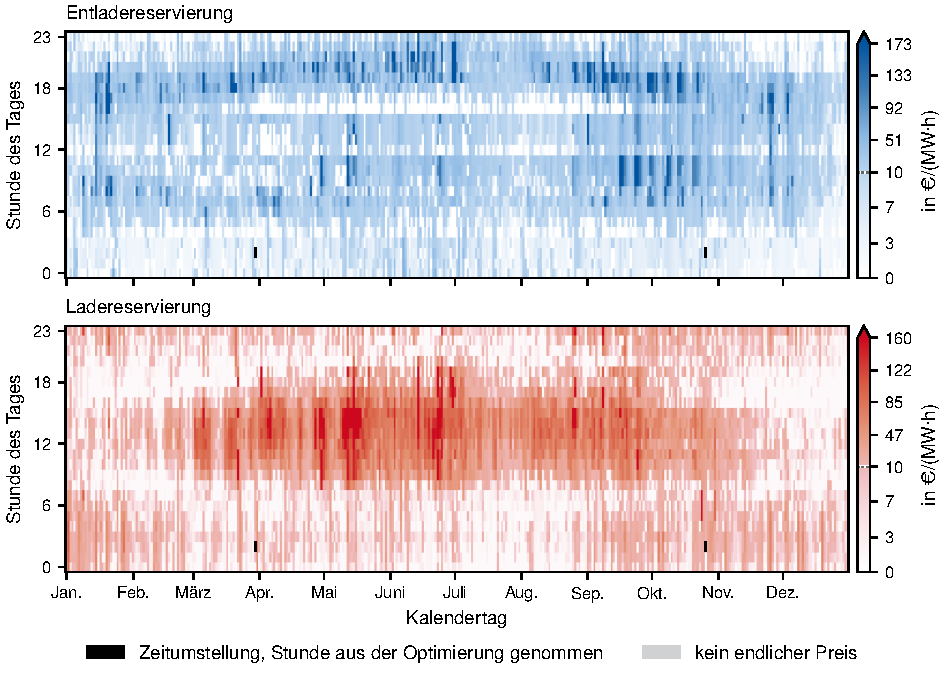
\includegraphics[width=\textwidth]{figures/chapter_4/heatmap_reservierungspreis_2025.pdf}
    \caption{Kurativer Reservierungspreis je Stunde und Kalendertag im Jahr 2025, oben die Entlade- und unten die Ladereservierung.}
    \label{fig:heatmap_reservierungspreis}
\end{figure}

% ---------------------------------------------------------------
\section{Kurativer Reservierungspreis und Engpassbedarf}
\label{sec:price_vs_redispatch}
% [Ziel: 2 Seiten]
%
% KERNAUSSAGE: Der kurative Reservierungspreis folgt dem Redispatchbedarf
% nicht, denn im Dezember trifft der niedrigste Preis auf den zweithoechsten
% Bedarf.
%
% ANSCHLUSS NACH VORN: Abschnitt 4.4 fragt, was die Summe dieser Stundenpreise
% gegenueber der uebrigen Vermarktung bedeutet.
%
% NICHT SAGEN: nicht, die kurative Vorhaltung sei deshalb guenstig oder
% lohnend, denn dieser Schluss verlangt den Nutzen und gehoert nach Kapitel 5.
% Nicht, der fehlende Zusammenhang gelte je Netzknoten, denn ausgewertet ist
% der deutschlandweite Redispatch.
%
% EIGENSTAENDIGE ABLEITUNG, vom Verfasser zu pruefen. Die Rangkorrelation
% zwischen Tagesmedian und Redispatchvolumen stammt aus eigener Rechnung vom
% 17.09.2026 und ist gegen die Aggregation im Skript jahreslauf_redispatch.py
% zu pruefen, bevor eine Zahl in den Text geht.

\begin{itemize}
    \item Anschluss, nämlich dass das Muster aus Abschnitt~\ref{sec:price_pattern} sagt, wann Vorhaltung teuer ist, und offen lässt, ob diese Stunden mit dem Bedarf zusammenfallen
    \item Aufbau der Abbildung~\ref{fig:jahreslauf_redispatch} in einem Satz, nämlich der Tagespreis als Band mit Median auf der linken und das Redispatchvolumen des Tages auf der rechten Achse
    \item Der Redispatchbedarf ist im Januar mit rund 2680\,\si{MW} im Mittel am größten und im August mit rund 510\,\si{MW} am kleinsten
    \item Der kurative Reservierungspreis ist im September und Oktober am größten und der Bedarf im Januar, Februar, November und Dezember, sodass die Maxima auseinanderfallen
    \item Der Rangkorrelationskoeffizient zwischen dem Tagesmedian des Preises und dem Redispatchvolumen des Tages bleibt unter 0,25 und zeigt damit keinen Zusammenhang
    \item Zuordnung der Richtungen, nämlich die Entladereservierung zum Redispatch nach oben und die Ladereservierung zum Redispatch nach unten, weil ein einspeisender Speicher ein hochgefahrenes Kraftwerk ersetzt
    \item Der spezifische Preis des heutigen präventiven Redispatch liegt bei 101 Euro je Megawattstunde, nämlich 3,08 Milliarden Euro Kosten geteilt durch 30,44 Terawattstunden bewegter Menge im Jahr 2025
    \item Dieser Vergleichswert ist ein Arbeitspreis je bewegter Megawattstunde und der kurative Reservierungspreis ein Leistungspreis je vorgehaltener Megawattstunde, weshalb die Abbildung beide nebeneinanderstellt und nicht gegeneinander aufrechnet
    \item Folge für die Auswertung, nämlich dass der kurative Reservierungspreis eine Eigenschaft der Vermarktung und nicht des Netzzustands ist
\end{itemize}

% ABBILDUNG 4.2. Die Analysefassung liegt als
% analysen/03_breakeven/jahreslauf/jahreslauf_redispatch_2025.png vor. Zu tun
% bleibt: Umstellung auf die zweite Iteration nach Entscheidung E2, Textbreite,
% Achsenbeschriftung von Breakeven auf kurativer Reservierungspreis nach
% CLAUDE.md Abschnitt 5.
\begin{figure}[htbp]
    \centering
    % ABBILDUNGSLIEFERUNG am 21.09.2026, Anweisung aus bess_dispatch_optimization (ANWEISUNG_LIEFERUNG_ABBILDUNGEN.md, Stand 21.09.2026 16:14): Abbildung geliefert, Platzhalter ersetzt. Alte Zeile:
%    \platzhalterabb{Kurativer Reservierungspreis je Tag des Jahres 2025 als Band von Minimum bis Maximum mit Median, links in Euro je Megawatt und Stunde, daneben das Redispatchvolumen des Tages in Megawatt auf der rechten Achse, oben die Entlade- und unten die Ladereservierung.}
    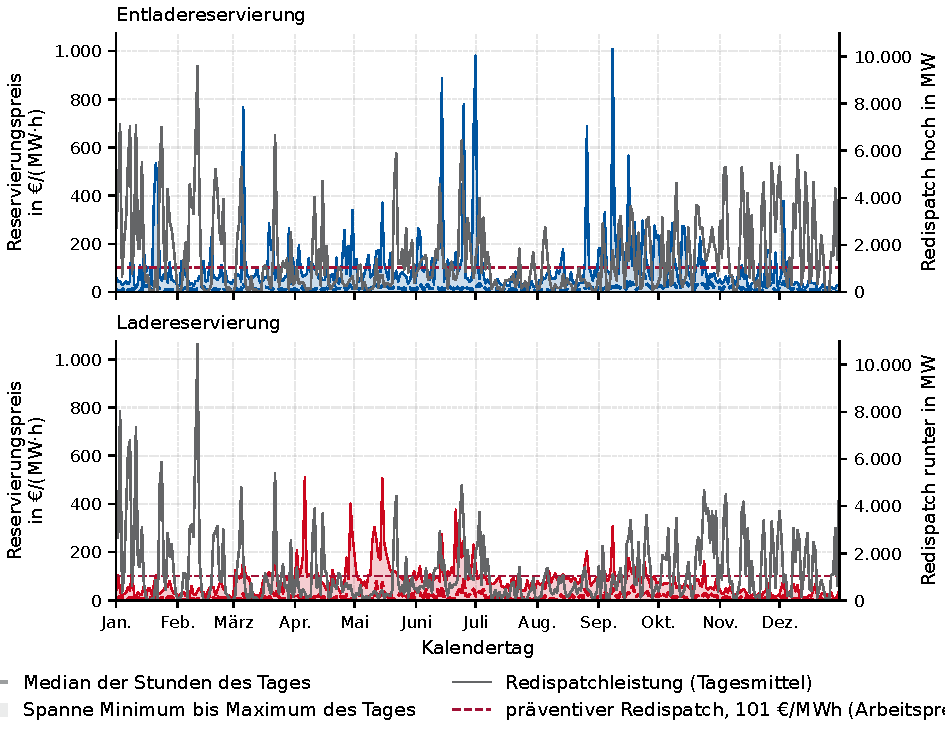
\includegraphics[width=\textwidth]{figures/chapter_4/jahreslauf_reservierungspreis_redispatch_2025.pdf}
    % ABBILDUNGSLIEFERUNG am 21.09.2026, Anweisung aus bess_dispatch_optimization (ANWEISUNG_LIEFERUNG_ABBILDUNGEN.md, Stand 21.09.2026 16:14), Abschnitt 7: die Linie bei 101 Euro je Megawattstunde ist der Arbeitspreis (3,08 Mrd. Euro auf 30,44 TWh) und kein Leistungspreis. Alte Fassung:
%    \caption{Kurativer Reservierungspreis je Tag des Jahres 2025 neben dem Redispatchvolumen des Tages.}
    \caption{Kurativer Reservierungspreis je Tag des Jahres 2025 neben der Redispatchleistung im Tagesmittel, zweite Iteration, die waagerechte Linie ist der Arbeitspreis des präventiven Redispatch 2025.}
    \label{fig:jahreslauf_redispatch}
\end{figure}

% ---------------------------------------------------------------
\section{Zahlung bei vollständiger Bindung}
\label{sec:full_binding_cost}
% [Ziel: 2,5 Seiten]
%
% KERNAUSSAGE: Eine durchgehende Reservierung des ganzen Jahres kostet mehr als
% den Referenzerloes, weil jede Stunde ihren eigenen Grenzpreis fuer die volle
% Leistung erhaelt, waehrend die Anlage ihren Erloes an Stundenpaaren verdient.
%
% ANSCHLUSS NACH VORN: Abschnitt 4.5 fragt, welche Vermarktung die Reservierung
% verdraengt, und damit, woran der Preis haengt.
%
% NICHT SAGEN: nicht, die kurative Reservierung sei damit zu teuer oder
% unwirtschaftlich, denn dafuer fehlt der Nutzen. Nicht, ein Tagesprodukt waere
% besser, denn das ist eine Empfehlung und gehoert nach Abschnitt 5.5.
%
% HIER STEHT DIE ERSTE ITERATION, nach Entscheidung E2, weil der Unterschied
% zwischen den Iterationen die Aussage traegt.

\begin{itemize}
    \item Anschluss, nämlich dass die Abschnitte~\ref{sec:price_level} bis~\ref{sec:price_vs_redispatch} den Preis je Stunde zeigen und offen lassen, was die Summe dieser Preise bedeutet
    \item Aufbau der Abbildung~\ref{fig:erloesvergleich} in einem Satz und Definition der drei ausgewiesenen Größen
    \item Der Referenzerlös des Jahres 2025 beträgt 34,67 Millionen Euro für die betrachtete Anlage
    \item Unter dem Preisvektor der zweiten Iteration zahlt der \ac{ÜNB} 42,02 Millionen Euro für die Vorhaltung, und die Anlage verdient daneben noch 0,25 Millionen Euro an den übrigen Märkten
    \item Die Zahlung liegt damit um 21,9 Prozent über dem Referenzerlös
    \item Je Tag liegt der Abstand im Median bei 19,6 Prozent und im 90-Prozent-Quantil bei 48,8 Prozent, weshalb die Jahreszahl keinen Durchschnittstag beschreibt
    \item Die Ursache liegt im Stundenprodukt, denn jede Stunde erhält ihren Grenzpreis für die volle Leistung, während sich der verdrängte Erlös aus Arbitrage auf ein Paar aus Lade- und Entladestunde verteilt und beide Stunden dieselbe Preisspanne spiegeln
    \item Der Preisvektor der ersten Iteration verdrängt die übrige Vermarktung nicht vollständig, denn die Anlage verdient daneben 9,31 Millionen Euro, und die Summe aus Zahlung und Markterlös übersteigt den Referenzerlös um 45,1 Prozent
    \item Folge für die Wahl der Messgröße, nämlich dass die zweite Iteration die vollständigere Verdrängung bei geringerer Zahlung liefert
    \item Der ausgewiesene Preisvektor ist ein koordinatenweises und kein globales Minimum, und die umgekehrte Reihenfolge des Abstiegs liegt an den beiden vermessenen Tagen um 5,5 und 17,7 Prozent darunter
    \item Folge für die Lesart der Zahl, nämlich dass sie die vorsichtigere Seite einer gemessenen Spanne ist
\end{itemize}

% ABBILDUNG 4.3. Die Schriftfassung liegt vor, erzeugt von
% analysen/code/schrift/13_erloesvergleich/erloesvergleich_vollverdraengung.py.
% ZU TUN VOR ABGABE: Die Achse traegt heute Erloes 2025 [Mio. Euro], netto nach
% Degradation. Sie ist auf Erloes in Mio. Euro zu kuerzen, und das Jahr sowie
% der Zusatz netto nach Degradation gehoeren in die Bildunterschrift. Die Zahl
% der Tage ist gegen den Gesamtlauf zu pruefen, siehe N4.
\begin{figure}[htbp]
    \centering
    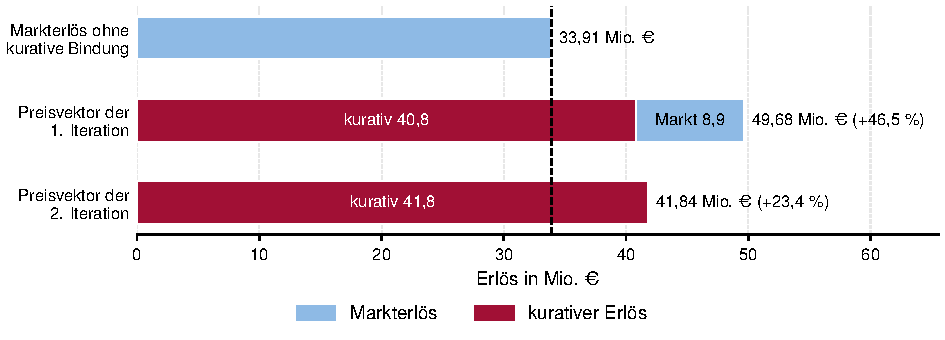
\includegraphics[width=\textwidth]{figures/chapter_4/erloesvergleich_vollverdraengung_2025.pdf}
    \caption{Erlös des Jahres 2025 ohne kurative Bindung und unter den Preisvektoren beider Iterationen, netto nach Degradation.}
    \label{fig:erloesvergleich}
\end{figure}

% ---------------------------------------------------------------
\section{Sensitivitätsanalyse}
\label{sec:sensitivities}
% [Ziel: 5 Seiten, davon 0,5 fuer die Einleitung und je 1,5 fuer die drei
% Unterabschnitte]
%
% AUFBAU DES ABSCHNITTS. Die drei Sensitivitaeten treten als drei Antworten auf
% eine Frage auf und nicht als Aufzaehlung von Varianten. Der kurative
% Reservierungspreis ist ein Opportunitaetskostenpreis, und wovon er abhaengt,
% ist damit die Frage, welche Vermarktung die Reservierung verdraengt. Die
% Reihenfolge ist begruendet und nicht gesetzt, naemlich zuerst die Groesse mit
% der staerksten gemessenen Wirkung, dann die Groesse, ueber die der UENB
% entscheidet, zuletzt die Groesse, ueber die der Betreiber entscheidet.
%
% ENTFALLENE SENSITIVITAETEN. Die alte Fassung fuehrte Abrufhaeufigkeit,
% Verguetungsniveau und Hoehe der Poenale. Alle drei sind durch die
% Entscheidungen zur Abrufwahrscheinlichkeit, zur gesuchten Groesse und zur
% Poenale gestrichen, siehe den offenen Punkt 21 des Protokolls. Die
% Anlagenauslegung ist nicht gerechnet. Der Degradationssatz und die
% Mindestgroesse sind gerechnet, bleiben hier aber aussen vor, weil Abschnitt
% 3.3.3 die Mindestgroesse schon traegt.

\begin{itemize}
    \item Überleitung, nämlich dass der kurative Reservierungspreis die Opportunitätskosten der zuletzt reservierten Leistung misst und damit an der verdrängten Vermarktung hängt
    \item Drei Größen kommen dafür in Betracht, nämlich die Modellierung der \ac{aFRR}, die Abrufdauer und der Spread am \ac{IDC}
    \item Begründung der Reihenfolge in einem Satz
    \item Die drei Sensitivitäten rechnen nicht über denselben Zeitraum, weshalb jede Bildunterschrift ihre Grundgesamtheit nennt
\end{itemize}

% ---------------------------------------------------------------
\subsection{Modellierung der \acs{aFRR}}
\label{sec:sensi_afrr}
% [Ziel: 1,5 Seiten]
%
% KERNAUSSAGE: Die Abbildung der aFRR im Modell bewegt den kurativen
% Reservierungspreis um mehr als das Dreifache, weil die aFRR und nicht der
% Energiemarkt die verdraengte Vermarktung ist.
%
% NICHT SAGEN: nicht, das Modell ueberschaetze oder unterschaetze den Preis,
% denn die Richtung der Verzerrung gehoert nach Abschnitt 5.4.

\begin{itemize}
    \item Anschluss, nämlich dass die \ac{aFRR} unter den geführten Märkten den größten Erlösbeitrag trägt und ihre Abbildung nach Abschnitt~\ref{sec:input_data} mehrere zulässige Formen hat
    \item Welche Größen variiert werden, nämlich die Preisquelle der Leistung und der Liefermodus der Arbeit
    \item Aufbau der Abbildung~\ref{fig:sensi_afrr} in einem Satz, nämlich Median und Band der mittleren 50 Prozent je Variante
    \item Ergebnis am 15.05.2025 in der Laderichtung, nämlich 37,9\,\EurMWh{} ohne \ac{aFRR}, 111,7\,\EurMWh{} mit dem mengengewichteten Mittelpreis und 265,1\,\EurMWh{} mit dem höchsten Zuschlag
    \item Ergebnis am 26.08.2025 in derselben Richtung, nämlich 19,5, 59,9 und 77,8\,\EurMWh{}
    \item Die Wirkung des Liefermodus der Arbeit ist kleiner als die der Preisquelle der Leistung, weshalb der Leistungspreis und nicht die gelieferte Arbeit die Opportunität setzt
    \item Folge für die Lesart der übrigen Ergebnisse, nämlich dass der Basisfall mit dem mengengewichteten Mittelpreis rechnet und der höchste Zuschlag nach Abschnitt~\ref{sec:input_data} allein eine Sensitivität ist
    \item Folge für den Vergleich, nämlich dass die Spanne der Modellierung größer ist als die Spanne der beiden folgenden Sensitivitäten
\end{itemize}

% ABBILDUNG 4.4. Zu bauen aus den Breakeven-Tabellen der Sensitivitaet
% sensi3_preis_mode, ohne neue Rechnung. Format wie Abbildung 4.5, naemlich
% Median, arithmetisches Mittel und Band der mittleren 50 Prozent je Variante,
% Entlade- und Ladereservierung nebeneinander. Grundgesamtheit sind die
% Analysetage und nicht das Jahr, was die Bildunterschrift nennt. Acht
% Varianten sind viel, weshalb die zweite Preisquelle in den Anhang kann.
\begin{figure}[htbp]
    \centering
    % ABBILDUNGSLIEFERUNG am 21.09.2026, Anweisung aus bess_dispatch_optimization (ANWEISUNG_LIEFERUNG_ABBILDUNGEN.md, Stand 21.09.2026 16:14): Abbildung geliefert, Platzhalter ersetzt. Alte Zeile:
%    \platzhalterabb{Kurativer Reservierungspreis je Variante der aFRR-Modellierung, Median und Band der mittleren 50 Prozent, Entlade- und Ladereservierung nebeneinander, über die Analysetage.}
    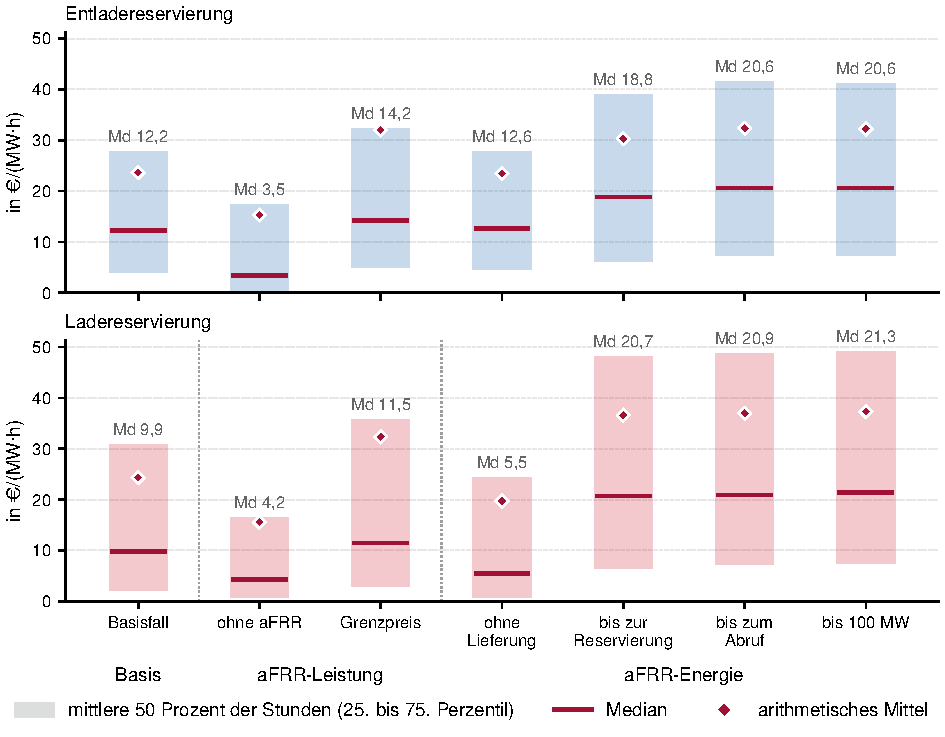
\includegraphics[width=\textwidth]{figures/chapter_4/sensi_afrr_modellierung_2025.pdf}
    % ABBILDUNGSLIEFERUNG am 21.09.2026, Anweisung aus bess_dispatch_optimization (ANWEISUNG_LIEFERUNG_ABBILDUNGEN.md, Stand 21.09.2026 16:14), Abschnitt 5: sieben Jahreslaeufe statt vier gepoolter Analysetage, Datei sensi_afrr_modellierung_2025.pdf. Alte Fassung:
%    \caption{Kurativer Reservierungspreis je Variante der \acs{aFRR}-Modellierung über die Analysetage.}
    \caption{Kurativer Reservierungspreis je Variante der \acs{aFRR}-Modellierung über alle Stunden des Jahres 2025, zweite Iteration.}
    \label{fig:sensi_afrr}
\end{figure}

% ---------------------------------------------------------------
\subsection{Abrufdauer und Breite des Ladezustandsbandes}
\label{sec:sensi_abrufdauer}
% [Ziel: 1,5 Seiten]
%
% KERNAUSSAGE: Eine kuerzere Abrufdauer senkt den kurativen
% Reservierungspreis kaum, denn der Effekt, den die erste Iteration zeigt, ist
% weitgehend eine Eigenschaft der stundenweisen Betrachtung.
%
% BEGRIFF, offene Entscheidung N3. Die Sensitivitaet variiert im Modell die
% Groesse kur_t_res, die der Quelltext als Abrufdauer der Energiebindung
% bezeichnet. Sie setzt die Breite des reservierten Ladezustandsbandes,
% naemlich eine Megawattstunde je Megawatt bei einer Stunde. Die BINDUNGSDAUER
% bleibt in allen Varianten eine Stunde, weil die Reservierung nach Abschnitt
% 3.1.2 ueber eine Zeitscheibe konstant ist. Das Modellrepository nennt die
% Sensitivitaet Vorhaltedauer, und die alte Fassung dieses Kapitels nannte sie
% Bindungsdauer. Beide Bezeichnungen traefen den gerechneten Fall nicht.
% Vorschlag deshalb Abrufdauer, im Einklang mit der Entscheidung zum Basisfall.
%
% NICHT SAGEN: nicht, der UENB solle die Abrufdauer so oder so waehlen, denn
% die Empfehlung gehoert nach Abschnitt 5.5. Nicht, das Ladezustandsband sei
% unerheblich, denn bei Teilreservierung wirkt es.

\begin{itemize}
    \item Anschluss, nämlich dass die Abrufdauer die einzige der drei Größen ist, über die der \ac{ÜNB} entscheidet, weil sie aus der Zeit folgt, die er die Maßnahme braucht
    \item Was die Abrufdauer im Modell verändert, nämlich die Breite des reservierten Ladezustandsbandes nach Abschnitt~\ref{sec:input_data} und nicht die Bindungsdauer
    \item Gerechnet sind eine Stunde als Basisfall sowie eine halbe und eine Viertelstunde, jeweils über alle Tage des Jahres 2025
    \item Aufbau der Abbildung~\ref{fig:sensi_abrufdauer} in einem Satz, im Format der Abbildung~\ref{fig:sensi_afrr}
    \item In der ersten Iteration senkt die Viertelstunde den Median deutlich, nämlich um 15 Prozent in der Entlade- und um 32 Prozent in der Laderichtung
    \item Nach der zweiten Iteration verschwindet der Effekt nahezu, denn die Zahlung der vollständigen Bindung ändert sich nicht
    \item Die Erklärung, nämlich dass bei einem vollständig gebundenen Tag ohnehin keine Leistung für andere Märkte frei steht und die Breite des Bandes deshalb keine weitere Vermarktung verdrängt
    \item Folge für das Produkt im beschreibenden Sinn, nämlich dass die Abrufdauer den Preis der vollständigen Bindung nicht bestimmt
    \item Folge für das Verfahren, nämlich dass ein Befund aus der ersten Iteration nicht auf die zweite übertragbar ist
\end{itemize}

% ABBILDUNG 4.5. Gebaut als
% analysen/05_sensitivitaet/tie_fighter_vorhaltedauer_2025.pdf, zeigt aber die
% erste Iteration, weil die Variantentabellen be_full_pos und be_full_neg bis
% zum 17.09.2026 nicht mitschrieben. Nach Schritt 8 des Gesamtlaufs ist die
% Fassung der zweiten Iteration zu zeichnen. Ein Feld mit beiden Richtungen
% genuegt. Soll der Gegensatz der Iterationen selbst die Aussage sein, sind es
% zwei Felder. Keine Whisker fuer Minimum und Maximum, weil sie ueber alle
% Varianten gleich sind.
\begin{figure}[htbp]
    \centering
    % ABBILDUNGSLIEFERUNG am 21.09.2026, Anweisung aus bess_dispatch_optimization (ANWEISUNG_LIEFERUNG_ABBILDUNGEN.md, Stand 21.09.2026 16:14): Abbildung geliefert, Platzhalter ersetzt. Alte Zeile:
%    \platzhalterabb{Kurativer Reservierungspreis je Abrufdauer von einer Stunde, einer halben und einer Viertelstunde, Median und Band der mittleren 50 Prozent, Entlade- und Ladereservierung nebeneinander, über alle Stunden des Jahres 2025.}
    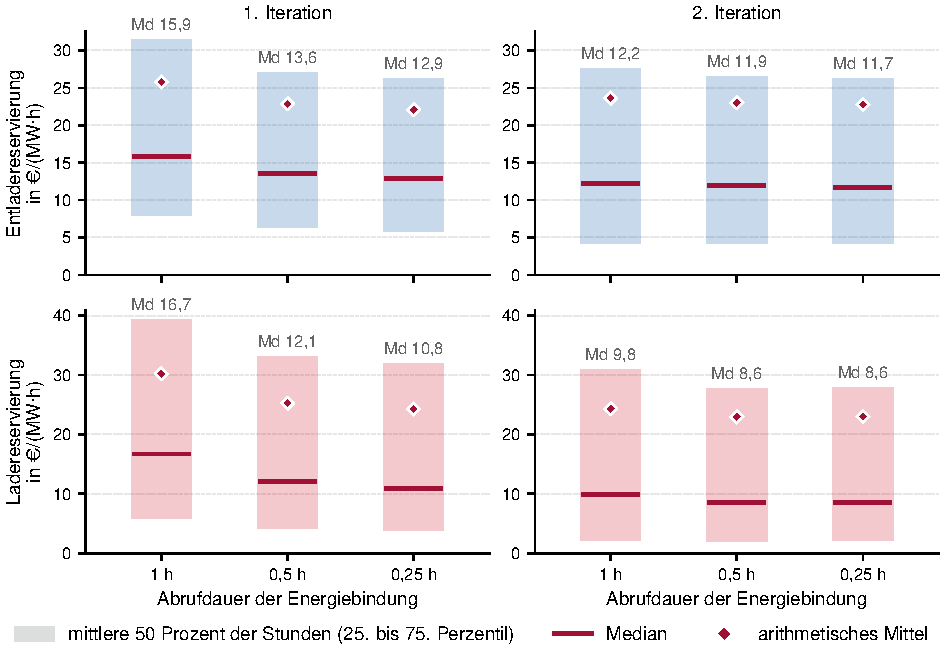
\includegraphics[width=\textwidth]{figures/chapter_4/sensi_abrufdauer_2025_iterationen.pdf}
    % ABBILDUNGSLIEFERUNG am 21.09.2026, Anweisung aus bess_dispatch_optimization (ANWEISUNG_LIEFERUNG_ABBILDUNGEN.md, Stand 21.09.2026 16:14), Abschnitt 6: zwei Fassungen geliefert, Vorschlag von Fable ist die Fassung mit beiden Iterationen (sensi_abrufdauer_2025_iterationen.pdf), weil sie den Befund traegt; die Zweifeldfassung liegt als sensi_abrufdauer_2025.pdf daneben, Entscheidung des Verfassers offen. Alte Fassung:
%    \caption{Kurativer Reservierungspreis je Abrufdauer über alle Stunden des Jahres 2025.}
    \caption{Kurativer Reservierungspreis je Abrufdauer über alle Stunden des Jahres 2025, links die erste und rechts die zweite Iteration, oben die Entlade- und unten die Ladereservierung.}
    \label{fig:sensi_abrufdauer}
\end{figure}

% ---------------------------------------------------------------
\subsection{Spread am kontinuierlichen Intraday-Handel}
\label{sec:sensi_idc}
% [Ziel: 1,5 Seiten]
%
% KERNAUSSAGE: Ein um den Faktor zwei gestreckter Spread am IDC hebt den
% kurativen Reservierungspreis nur wenig, weil die Regelleistungsmaerkte die
% Opportunitaet setzen, sobald sie teurer sind.
%
% NICHT SAGEN: nicht, der kurative Marktmechanismus sei gegen strategisches
% Bieten geschuetzt, denn das Modell bildet nach Abschnitt 3.2.2 keinen
% Bietwettbewerb ab. Dieser Schluss gehoert nach Abschnitt 5.2.
%
% OFFENE ENTSCHEIDUNG 6.4 der Planung, hier vorgeschlagen: Die Kurven ueber der
% Streckung bleiben, weil der Abstand der beiden Kurven der Befund ist und ein
% Band je Variante ihn nicht zeigt. Das gemeinsame Format gilt damit fuer die
% Abbildungen 4.4 und 4.5.

\begin{itemize}
    \item Anschluss, nämlich dass der Spread am \ac{IDC} die Größe ist, die ein Betreiber zu hoch ansetzen kann, weil ein Aufschlag nach Abschnitt~\ref{sec:input_data} den mehrfachen Handel bewertet und seine Höhe nicht beobachtbar ist
    \item Was variiert wird, nämlich die Streckung des Spreads um das Tagesmittel, sodass das Preisniveau bleibt und allein die Handelsspanne wächst
    \item Aufbau der Abbildung~\ref{fig:sensi_idc} in einem Satz, die anders als die Abbildungen~\ref{fig:sensi_afrr} und~\ref{fig:sensi_abrufdauer} Kurven über der Streckung zeigt
    \item Ergebnis ohne die Märkte für Regelleistung am 11.02.2025, nämlich ein Anstieg in der Entladerichtung von 9,1 auf 21,4\,\EurMWh{}
    \item Ergebnis mit allen geführten Märkten am selben Tag, nämlich ein Anstieg von 11,6 auf 21,4\,\EurMWh{}, wobei sich der Abstand beider Kurven mit steigender Streckung schließt
    \item Der Abstand beider Kurven ist der Befund, nämlich dass die \ac{aFRR} die Opportunität setzt, solange sie über dem gestreckten Spread liegt
    \item Damit führt die dritte Sensitivität auf die erste zurück, und die drei Sensitivitäten tragen zusammen eine Aussage
    \item Vorbehalt zur Grundgesamtheit, nämlich fünf Beispieltage für die Mechanik und ein Jahreslauf für die Tragweite
    \item Vorbehalt zur Aussage, nämlich dass ein steigender Preis ohne zusätzlich belegte Stunden allein eine Buchung wäre
\end{itemize}

% ABBILDUNG 4.6. Die Analysefassung liegt als
% analysen/05_sensitivitaet/idc_hebel.pdf vor, mit fuenf Tagesfeldern und einem
% Jahresfeld. Das Jahresfeld braucht einen Jahreslauf mit der Streckung zwei,
% und die vorhandene Datei heatmap_daten_2025_lam20.parquet stammt aus dem
% Stand vor der Kausalitaetsbedingung und vor der Korrektur der
% Zeitumstellung. Ohne neuen Jahreslauf traegt die Abbildung allein die
% Tagesfelder, was die Bildunterschrift dann nennen muss.
\begin{figure}[htbp]
    \centering
    % ABBILDUNGSLIEFERUNG am 21.09.2026, Anweisung aus bess_dispatch_optimization (ANWEISUNG_LIEFERUNG_ABBILDUNGEN.md, Stand 21.09.2026 16:14): Abbildung geliefert, Platzhalter ersetzt. Alte Zeile:
%    \platzhalterabb{Kurativer Reservierungspreis über der Streckung des Spreads am IDC von eins bis zwei, je Beispieltag ein Feld, mit und ohne die Märkte für Regelleistung, Median je Richtung.}
    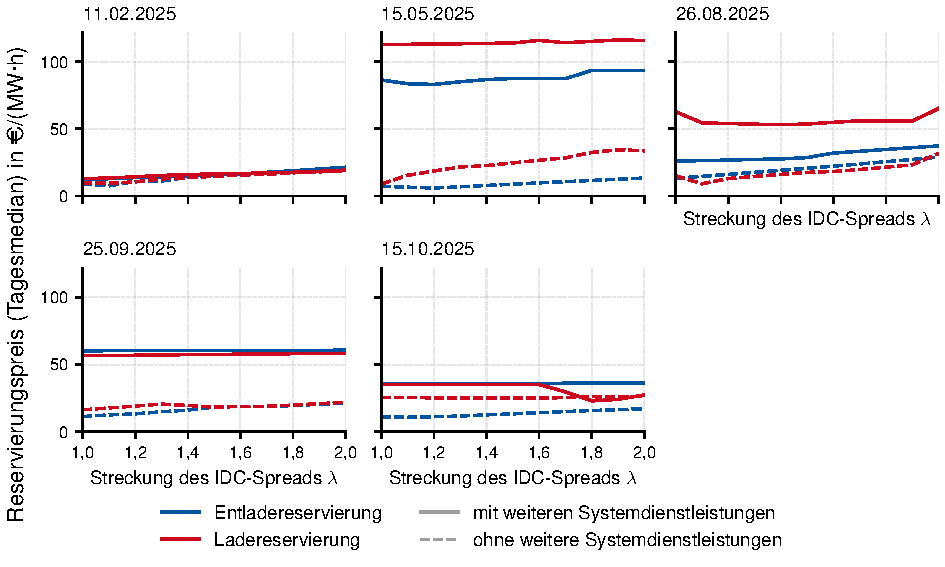
\includegraphics[width=\textwidth]{figures/chapter_4/sensi_idc_spread.pdf}
    % ABBILDUNGSLIEFERUNG am 21.09.2026, Anweisung aus bess_dispatch_optimization (ANWEISUNG_LIEFERUNG_ABBILDUNGEN.md, Stand 21.09.2026 16:14), Abschnitt 7: fuenf Beispieltage, erste Iteration, kein Jahresfeld. Alte Fassung:
%    \caption{Kurativer Reservierungspreis über der Streckung des Spreads am \acs{IDC}, mit und ohne die Märkte für Regelleistung.}
    \caption{Kurativer Reservierungspreis über der Streckung des Spreads am \acs{IDC} an fünf Beispieltagen, mit und ohne die Märkte für Regelleistung, Median je Richtung, erste Iteration.}
    \label{fig:sensi_idc}
\end{figure}

% ---------------------------------------------------------------
\section{Zusammenfassung der Ergebnisse}
\label{sec:results_summary}
% [Ziel: 1 Seite]
%
% KERNAUSSAGE: Die Ergebnisse tragen zusammen die Aussage, dass der kurative
% Reservierungspreis ein Preis gegen die Regelleistung und nicht gegen die
% Arbitrage ist.
%
% NICHT SAGEN: keine Einordnung in die bestehenden Verguetungslogiken, keine
% Bewertung gegen den Anforderungskatalog, keine Empfehlung. Alle drei folgen
% in Kapitel 5.

\begin{itemize}
    \item Anschluss, nämlich dass die drei Sensitivitäten auf denselben Markt weisen
    \item Der kurative Reservierungspreis liegt im Median im niedrigen zweistelligen Bereich je Megawatt und Stunde, mit einem oberen Rand zwei Größenordnungen darüber
    \item Die volle Reservierung ist in nahezu jeder Stunde des Jahres 2025 erreichbar
    \item Der kurative Reservierungspreis folgt dem Tagesgang der Einspeisung und nicht dem Redispatchbedarf
    \item Die Zahlung bei durchgehender Bindung übersteigt den Referenzerlös um 21,9 Prozent, und die Ursache liegt im Stundenprodukt
    \item Der kurative Reservierungspreis hängt an der \ac{aFRR} und ist damit ein Preis gegen die Regelleistung
    \item Der ermittelte Wert ist der opportunitätskostenbasierte Teil eines Gebots und nicht das Gebot
\end{itemize}

% ===============================================================
% ALTE GLIEDERUNG vom 18.08.2026, ersetzt am 18.09.2026 durch die Sortierung
% aus KAPITEL_4_AUFBAU.md. NICHT WIEDER AUFNEHMEN. Gruende je Abschnitt:
%   4.1 Referenzfall und 4.2 Fahrplan unter Bindung stehen inzwischen in
%       Abschnitt 3.3 sowie in den Anhaengen zur Einzelmarktvalidierung und
%       zum Fahrplan ohne die Mindestgroesse. Als eigene Abschnitte
%       wiederholten sie Kapitel 3.
%   4.3 Die Zerlegung in entgangene Arbitrage und zusaetzlichen Werteverbrauch
%       folgt der Verguetungsstruktur der Festlegung und gehoert nach
%       Abschnitt 5.1.
%   4.4 Abrufhaeufigkeit, Verguetungsniveau und Poenalehoehe sind gestrichen,
%       siehe den offenen Punkt 21 des Protokolls. Der Kommentarblock unten,
%       der die Poenalehoehe als Sensitivitaet aufnimmt, ist damit UEBERHOLT.
%   4.5 Die gesuchte Groesse steht jetzt am Anfang des Kapitels und nicht auf
%       seiner letzten Seite.
% ---------------------------------------------------------------
% %%                       IAEW LaTeX Template                        %%
% %%%%%%%%%%%%%%%%%%%%%%%%%%%%%%%%%%%%%%%%%%%%%%%%%%%%%%%%%%%%%%%%%%%%%%
%
% \chapter{Exemplarische Anwendung und Ergebnisse}
% \label{ch:results}
% % ===============================================================
% % Zielumfang Kapitel 4: 16 Seiten
% %   4.1 Referenzfall ohne kurative Bindung ................... 3
% %   4.2 Fahrplaene und Ladezustandsverlaeufe unter Bindung ... 4
% %   4.3 Erloeswirkung und Opportunitaetskosten ............... 4
% %   4.4 Sensitivitaeten ...................................... 4
% %   4.5 Ableitung des kurativen Reservierungspreises ......... 1
% %
% % IN DIESEM KAPITEL NUR BESCHREIBEN, NICHT INTERPRETIEREN.
% % Das ist der häufigste Fehler bei dieser Kapitelaufteilung. Wer die
% % Trennung diszipliniert durchhält, schreibt Kapitel 5 fast von selbst.
% %
% % ENTSCHEIDUNGEN VOM 18.08.2026, verbindlich fuer dieses Kapitel:
% %   1  Die gesuchte Groesse heisst kurativer Reservierungspreis.
% %      Mindestverguetung und Erloesdifferenz werden nicht verwendet.
% %   2  Der modifizierte Weber-Ansatz wird nicht nachgerechnet. Die
% %      frueher in 4.3 vorgesehene Gegenueberstellung mit der Verguetung
% %      nach diesem Ansatz ist entfallen, weil ohne Nachrechnung keine
% %      Zahl vorliegt, gegen die gestellt werden koennte. Die Einordnung
% %      bleibt qualitativ in Abschnitt 5.1.
% %   3  Die Poenalehoehe ist als Sensitivitaet aufgenommen.
% % ===============================================================
%
% % ---------------------------------------------------------------
% \section{Referenzfall ohne kurative Bindung}
% \label{sec:reference_case}
% % [Ziel: 3 Seiten]
%
% \begin{itemize}
%     \item Marktoptimaler Fahrplan des Batteriespeichers am Beispieltag
%     \item Zyklenzahl, Erlöse je Markt, Auslastung des SoC-Bands
%     \item Plausibilisierung gegen die Preiszeitreihe
% \end{itemize}
%
% % ---------------------------------------------------------------
% \section{Fahrplan- und Ladezustandsverläufe unter kurativer Bindung}
% \label{sec:bound_case}
% % [Ziel: 4 Seiten]
%
% \begin{itemize}
%     \item Veränderung des Fahrplans gegenüber dem Referenzfall
%     \item Verlauf des Ladezustands und Ausnutzung des verbleibenden Bands
%     \item Verlagerung von Lade- und Entladevorgängen in andere Viertelstunden
% \end{itemize}
%
% % ---------------------------------------------------------------
% \section{Erlöswirkung und Opportunitätskosten}
% \label{sec:revenue_impact}
% % [Ziel: 4 Seiten]
%
% \begin{itemize}
%     \item Unterschied der Erlöse zwischen freiem und gebundenem Fahrplan
%     \item Aufteilung nach Märkten
%     \item Zerlegung in die entgangene Arbitrage und den zusätzlichen Werteverbrauch
% \end{itemize}
%
% % GESTRICHEN am 18.08.2026: Hier standen zwei Stichpunkte, naemlich die
% % Gegenueberstellung mit der Verguetung nach dem modifizierten
% % Weber-Ansatz und der getrennte Ausweis von Erzeugungsauslagen und
% % Optionswert. Beide setzen eine eigene Nachrechnung des fremden
% % Verfahrens voraus, die nicht stattfindet. Nicht wieder aufnehmen.
%
% % ---------------------------------------------------------------
% \section{Sensitivitätsanalyse}
% \label{sec:sensitivities}
% % [Ziel: 4 Seiten]
%
% \begin{itemize}
%     \item Abrufhäufigkeit
%     \item Vergütungsniveau
%     \item Bindungsdauer und Breite des reservierten Ladezustandsbands
%     \item Höhe der Pönale bei Nichterfüllung
%     \item Anlagenauslegung, also das Verhältnis von Energie zu Leistung
% \end{itemize}
%
% % ---------------------------------------------------------------
% \section{Ableitung des kurativen Reservierungspreises}
% \label{sec:reservation_price}
% % [Ziel: 1 Seite]
% %
% % Das Ergebnis ist als konservative Obergrenze zu benennen, denn mit
% % vollstaendiger Preiskenntnis trifft der unrestringierte Fahrplan jede
% % Preisspitze exakt, wodurch die Opportunitaetskosten der Bindung nach
% % oben verzerrt sind. Die Begruendung gehoert nach Abschnitt 5.4.
% % KEINE OBERGRENZE DES PREISES nennen, auch nicht verneinend. Der
% % Reservierungspreis ist der opportunitaetskostenbasierte Teil des
% % Gebots und nicht das Gebot selbst, weil eine Poenale zusaetzlich eine
% % Risikopraemie erzeugt.
